\documentclass[11pt]{article} 

\usepackage[utf8]{inputenc} 

\usepackage{graphicx}

\usepackage{geometry}
\geometry{a4paper} 


\title{Winterthur Yard: Projektidee}
\author{Maja Fritschi, Raphael Spörri, Florian Bosshard}
\date{} 
\begin{document}
\maketitle

\tableofcontents
\newpage

\section{Projektteam}
Das Projekt wird von folgenden Personen entwickelt:
\begin{itemize}
\item Maja Fritschi (fritsmaj)
\item Raphael Spörri (sporrra0)
\item Florian Bosshard (bosshflo)
\end{itemize}


\section{Spielbeschreibung}
In diesem Projekt wird eine Schnitzeljagd ähnlich dem Spiel Scotland Yard, durch die Winterthurer Altstadt entwickelt. Daher auch die ähnliche Projektbezeichnung Winterthur Yard. 
\\\\
Ziel des Spiels ist es, MisterX zu fangen, der sich an verschiedenen Punkten in der Altstadt versteckt. Hat man MisterX gefangen, verrät er einem ein Geheimnis, beispielsweise die Koordinaten eines Geocaches \footnote{Versteck des Spiels Geocaching, siehe http://www.geocaching.com}. 
\\
MisterX wird dabei durch einen Computerspieler dargestellt, der sich automatisch von Punkt zu Punkt bewegt. Der Spieler geht durch die Stadt und versucht MisterX zu finden. 
\\\\
Über die Karte ist ein Graph entlang den Strassen und Gassen der Altstadt gelegt. MisterX wechselt seinen Standort in einem definierten Zeitintervall und bewegt sich immer nur den Kanten zwischen den einzelnen Knoten entlang. In der Applikation kann die Funktion "MisterX fangen" aufgerufen werden sobald man physisch an einem der definierten Knoten ist. Mittels Geolocation gibt er dadurch an den einzelnen Knoten seinen Standort bekannt. Befindet er sich am selben Ort wie MisterX, so hat er das Spiel gewonnen. Ansonsten sieht er, wo sich MisterX als letztes aufgehalten hatte. Zudem wird ihm  angezeigt, wo sich andere Spieler bei deren letzten Anfrage befanden. So ist es möglich koordiniert miteinander vorzugehen.


\section{Ziele}
\begin{itemize}
\item Schöne Stellen in der Winterthurer Altstadt besuchen
\item Funktionalität des eigenen Mobiltelefons kennen lernen
\item Ein Rätsel für einen Geocache erstellen, das bis jetzt einzigartig ist
\end{itemize}


\section{Anwender}
MisterX soll die Koordinaten eines Geocaches verraten. Viele Geocacher sind sehr technikinteressiert. Daher ist davon auszugehen, dass die meisten ein internetfähiges Mobiltelefon mit einem aktuellen Browser besitzen. 
\\\\
Die Applikation wird mobil unter iOS und Android getestet, sollte aber unter grundsätzlich auf allen gängigen Geräten lauffähig sein. 

\section{Anwendungsfälle}
\subsection{Anfrage an einem Knoten}
Befindet sich der Spieler an einem Knoten, so kann er eine Anfrage an den Spielserver absetzen. Vom Server erhält er die vorhergehende Position von MisterX, sowie die letzte Abfrageposition der anderen Spieler. Stimmt die aktuelle Position von MisterX mit der eigenen Position überein, wird dem Spieler mitgeteilt, dass er MisterX gefunden hat. Befindet sich MisterX an einer anderen Position wird dem Spieler auf der Karte die Position angezeigt, an welcher  MisterX sich vor seiner letzten Verschiebung befand. Ebenso werden dem Spieler die letzten Abfragepositionen der übrigen Spieler angezeigt.
Befindet sich der Spieler nicht an einem Knoten, kann keine Anfrage abgesetzt werden.

\subsection{Anzeige der aktuellen Position}
Befindet sich der Spieler im Spielbereich wird diesem auf der Karte seine aktuelle Position angezeigt welche regelmässig aktualisiert wird. Für andere Spieler ist lediglich der letzte Anfrageort ersichtlich.

\subsection{Neue Teilnahme am Spiel}
Es existiert lediglich ein durchgehend laufendes Spiel auf dem Server an welchem der Spieler teilnehmen kann. 
Nach Eingabe des Spielernamens gelangt der Spieler auf die Karte mit dem Spiel-Graphen wo seine aktuelle Position angezeigt wird.
\\\\
Um mit dem Spiel beginnen zu können muss sich der Spieler zu einem Knoten begeben und eine erste Anfrage absetzen. Bis zu diesem Zeitpunkt sind noch keine Spielaktivitäten ersichtlich.
Für andere Spieler wird der neue Spieler erst ab der ersten Anfrage sichtbar.


\section{GUI}
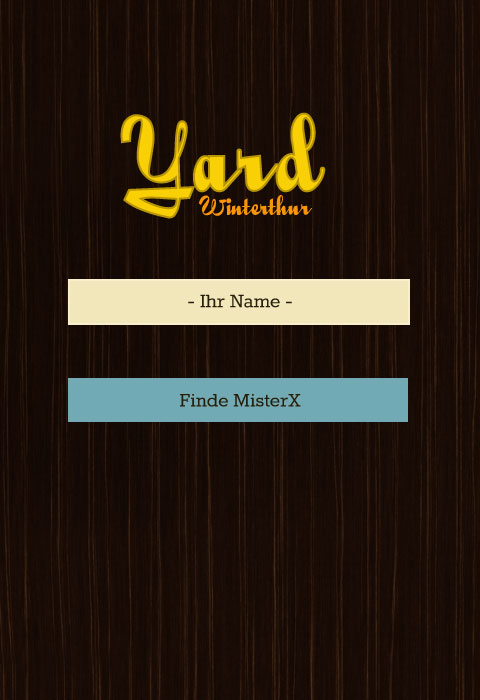
\includegraphics[width=8cm]{Bilder/homeView.jpg}
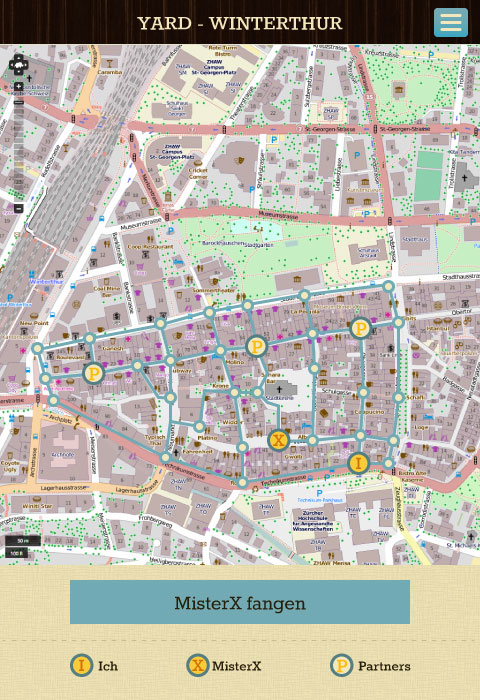
\includegraphics[width=8cm]{Bilder/karteView.jpg}
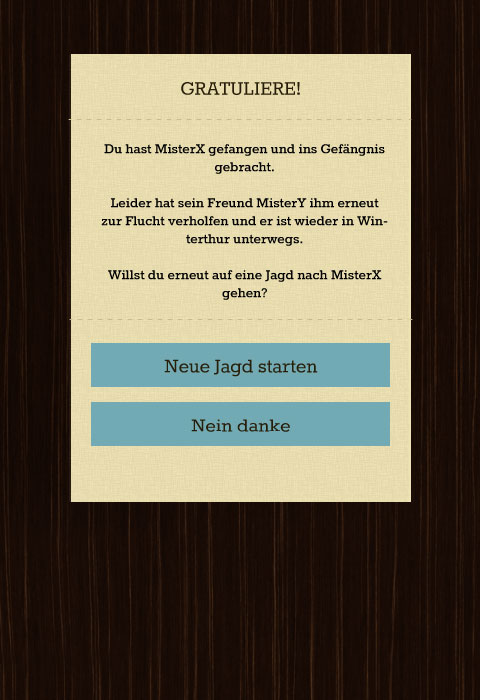
\includegraphics[width=8cm]{Bilder/gefundenView.jpg}
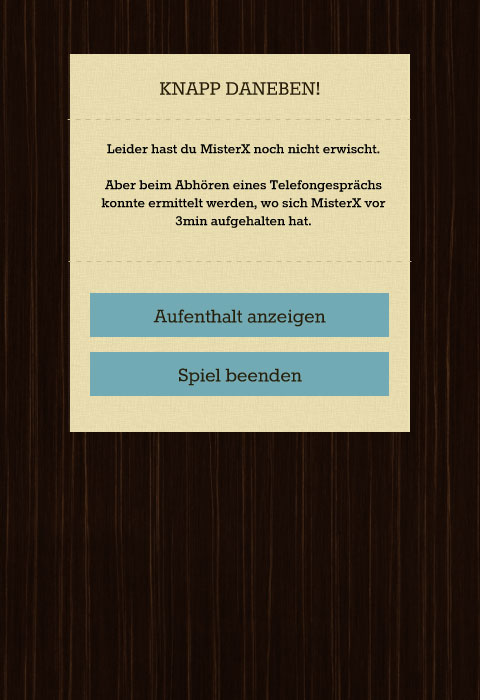
\includegraphics[width=8cm]{Bilder/danebenView.jpg}
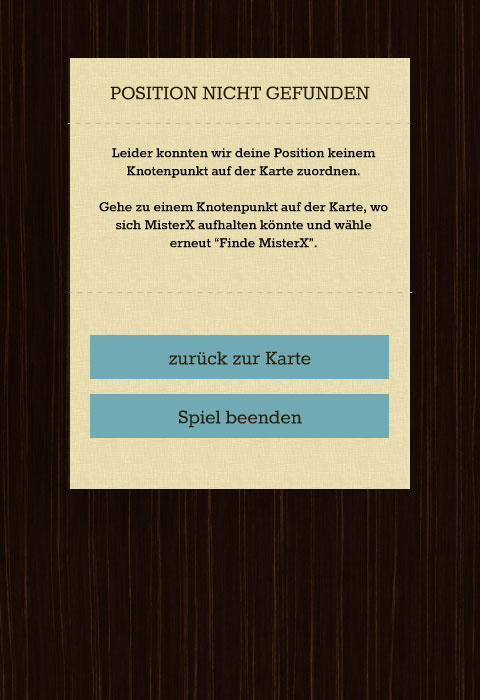
\includegraphics[width=8cm]{Bilder/keinePositionView.jpg}
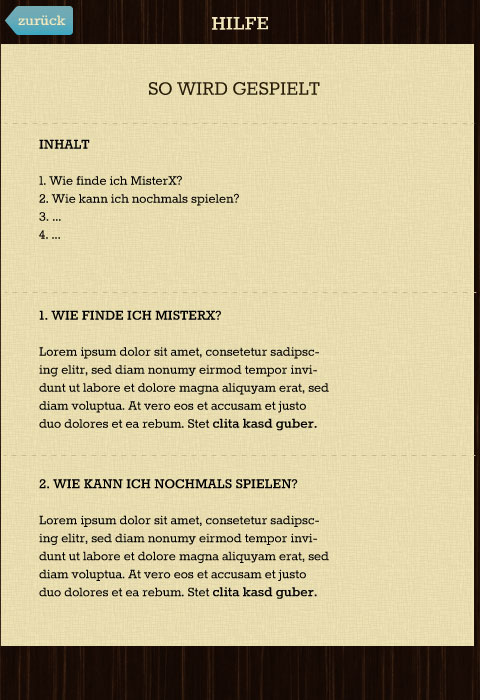
\includegraphics[width=8cm]{Bilder/hilfeView.jpg}

\includegraphics[width=8cm]{Bilder/ueberView.jpg}



\end{document}
